\documentclass[final]{beamer} 
\mode<presentation> {
  \usetheme{Berlin}
}

\usepackage{url}
\usepackage[utf8]{inputenc}
\usepackage{amsmath,amsthm, amssymb, latexsym}
\usefonttheme[onlymath]{serif}
\boldmath
%%\usepackage[size=custom,width=84.1,height=118.9,scale=2,orientation=portrait]{beamerposter}
\usepackage[size=A0,scale=2,orientation=portrait]{beamerposter}
\title{Guampa Poster}
\author{HLTDI}
\institute[Indiana University]{School of Informatics and Computing, Indiana University}
\date{May 29, 2014}
\begin{document}

\begin{frame}{} 
  \begin{block}
    {\centering \Huge Guampa: a Toolkit for Collaborative Translation}\par
    \centering
    {\large Alex Rudnick, Taylor Skidmore, Alberto Samaniego, and Michael Gasser}
    \par
  \end{block}

\begin{columns}[t]

%%% left column %%% 
  \begin{column}{.32\linewidth}

  \vfill
  %%\begin{block}{\large Contributions}
  \begin{block}{\large Introducing Guampa}
    \centering
    \begin{itemize}
    \item Software to support a community translating documents into
    under-served or heritage languages
    \item ... while building bitext corpora to support machine translation
    system training!
    \item Also supports discussions about translations so that users can help
    each other learn
    \item Designed in cooperation with educators in Paraguay for both online
    and classroom use
    \item Free Software, modifiable for your use case
    \item Features easy installation with setup instructions
    \end{itemize}
  \end{block}

  \centering
  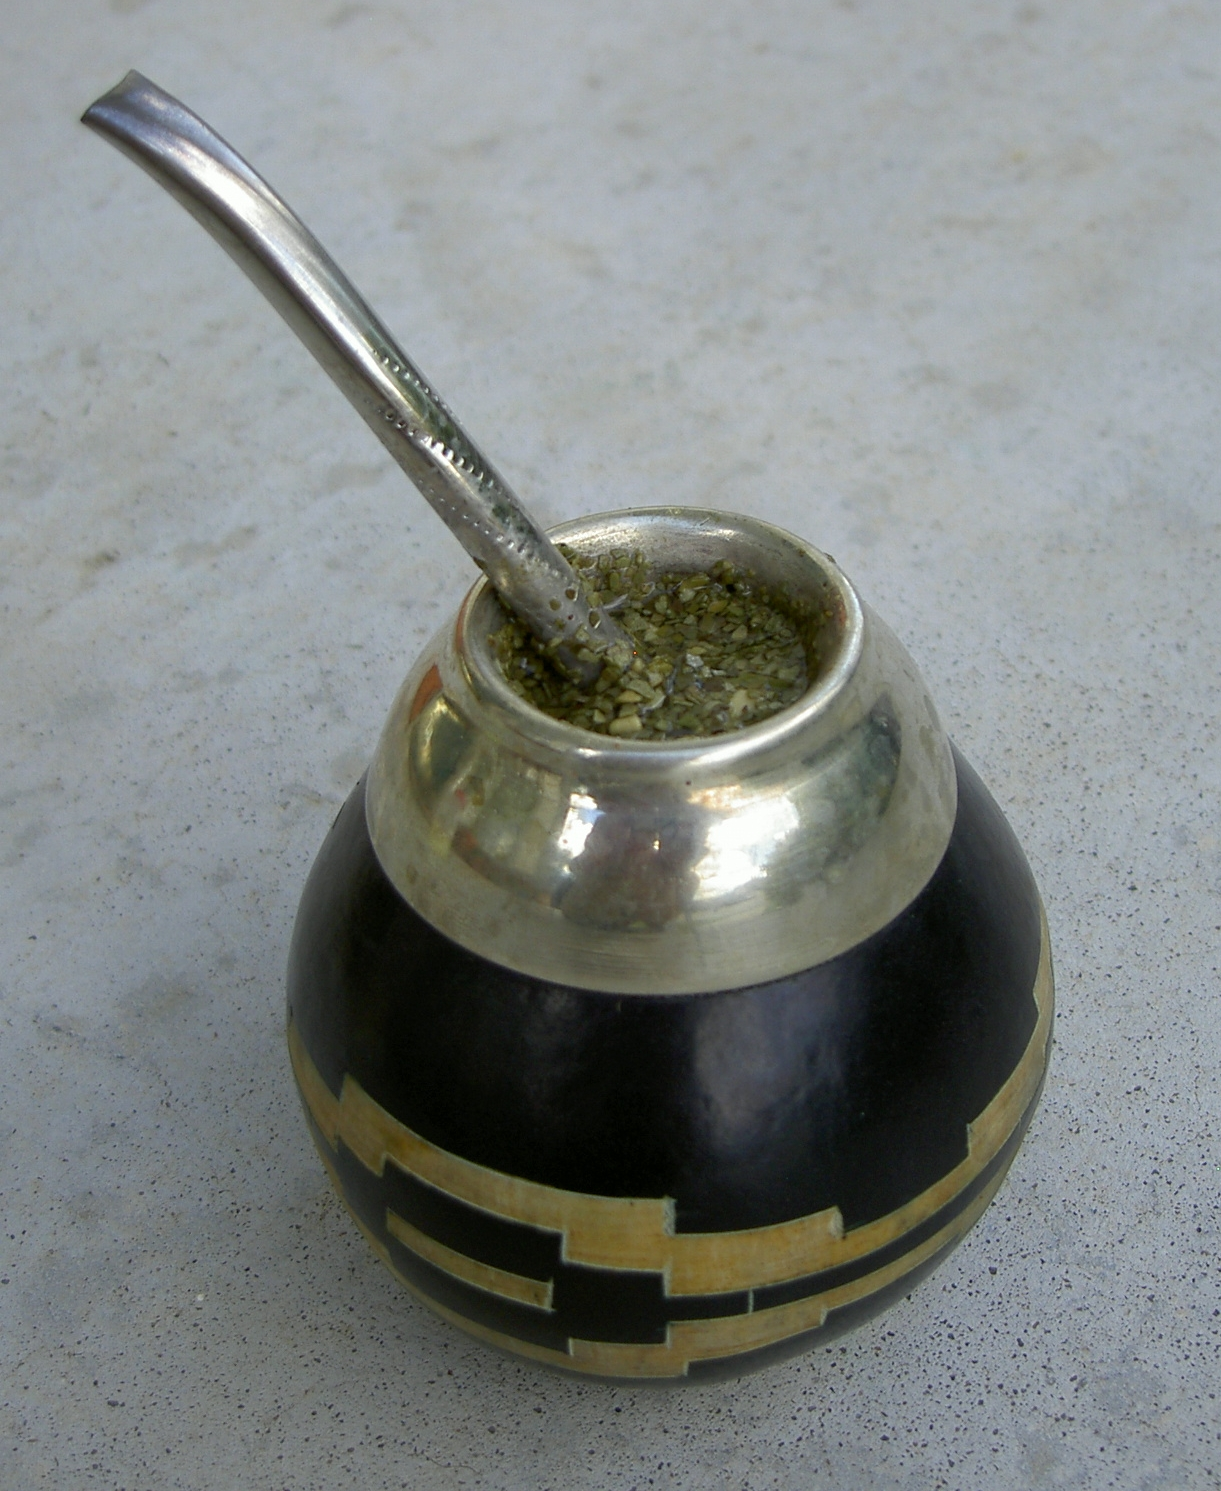
\includegraphics[width=.3\linewidth]{guampa_mate.jpg}

  \begin{block}{\large Importing Documents for Translation}
    \centering
    \begin{itemize}
    \item Automatic import of Wikipedia documents and export of translated texts
    \item Upload and tag documents to be translated
    \item Supports many document formats with Apache Tika: PDF, MS Word, plain
    text...
    \item Configurable sentence segmentation with NLTK
    \item Language-independent design, easy to set up and localize for your
    favorite language pair.
    \end{itemize}
  \end{block}

  \end{column}

  %%% middle column %%%
  \begin{column}{.32\linewidth}
  \vfill
  \begin{block}{\large Under-Resourced Languages}
    \begin{itemize}
    \item Roughly 7000 languages in the world -- how many do you speak?
    \item We want to support translation into languages with many speakers
    but not lots of data.
    \item Focusing on Paraguayan Guarani -- millions of speakers
    \end{itemize}
  \end{block}

  \definecolor{htmlgreen}{HTML}{008000}
  \centering
  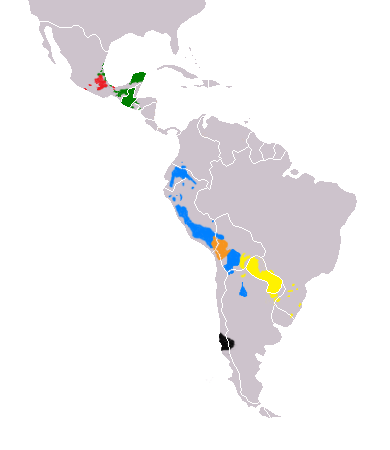
\includegraphics[width=.50\linewidth]{Map-Most_Widely_Spoken_Native_Languages_in_Latin_America.png}
  \begin{block}{\large Indigenous Languages of Latin America}
    \begin{tabular}{ll}
      {\color{blue}        $\blacksquare$} Quechua &
      {\color{yellow}      $\blacksquare$} Guarani \\
      {\color{orange}      $\blacksquare$} Aymara &
      {\color{red}         $\blacksquare$} Nahuatl \\
      {\color{htmlgreen}   $\blacksquare$} Mayan languages &
      {\color{black}       $\blacksquare$} Mapudungún \\
    \end{tabular}
  \end{block}

  \begin{block}{\large Open Source and Collaboration}
    \centering
    \begin{itemize}
    \item Working with educators in Paraguay
    \item Contributions and feedback welcome!
    \item \url{http://hltdi.github.io}
    \end{itemize}
  \end{block}


  \end{column}

  %%% right column %%%
  \begin{column}{.32\linewidth}

  \vfill

  \begin{block}{\large Translation Interface}
    \centering
    \begin{itemize}
    \item Integrated dictionaries to help learners
    \item Interface designed for online reading
    \item Features for supporting classes coming soon!
    \end{itemize}
  \end{block}

  \begin{block}{\large More Features}
    \begin{itemize}
    \item Easy login with \emph{Persona} from Mozilla
    \item Interface already translated into Paraguayan Spanish and US English.
    \item Language-independent design, easy to set up and localize for your
    favorite language pair. Currently in Spanish and English.
    \end{itemize}
  \end{block}

  \hfill
  \begin{block}{\large Future Work}
    \begin{itemize}
    \item Easy login with \emph{Persona} from Mozilla
    \item Access control, assigning translation as homework, and other features
    for supporting use in school classes coming soon!
    \end{itemize}
  \end{block}

  \hfill
  \begin{block}{\large HLTDI}
      \begin{itemize}
      \item is pronounced as:
      \end{itemize}
  \end{block}
  \begin{center}
    
\includegraphics[width=.30\linewidth]{hltdi-logo-small.png}
  \end{center}

  \end{column}
\end{columns}
\end{frame}
\end{document}
